%!TEX root = ../dissertation.tex

\graphicspath{{4-methods/figures/}}
\chapter{Methodology and Challenges}
\label{ch:methods}

The chapter outlines the prospective methodologies for this thesis and discusses the expected challenges in the proposed research directions.
It is unavoidable that the content of this chapter includes a certain degree of abstractness and ambiguity, because, as in most machine learning research, there is no predefined protocol for performing the research, and the very goal of this study lies on finding a methodology that works.
In light of this, the following section illustrates the high-level ideas, and the perspectives on generative models and the concept of disentanglement are presented, followed by the description of the evaluation metrics and the datasets to be used in the research.


\section{The High-Level Ideas}

\begin{figure}
	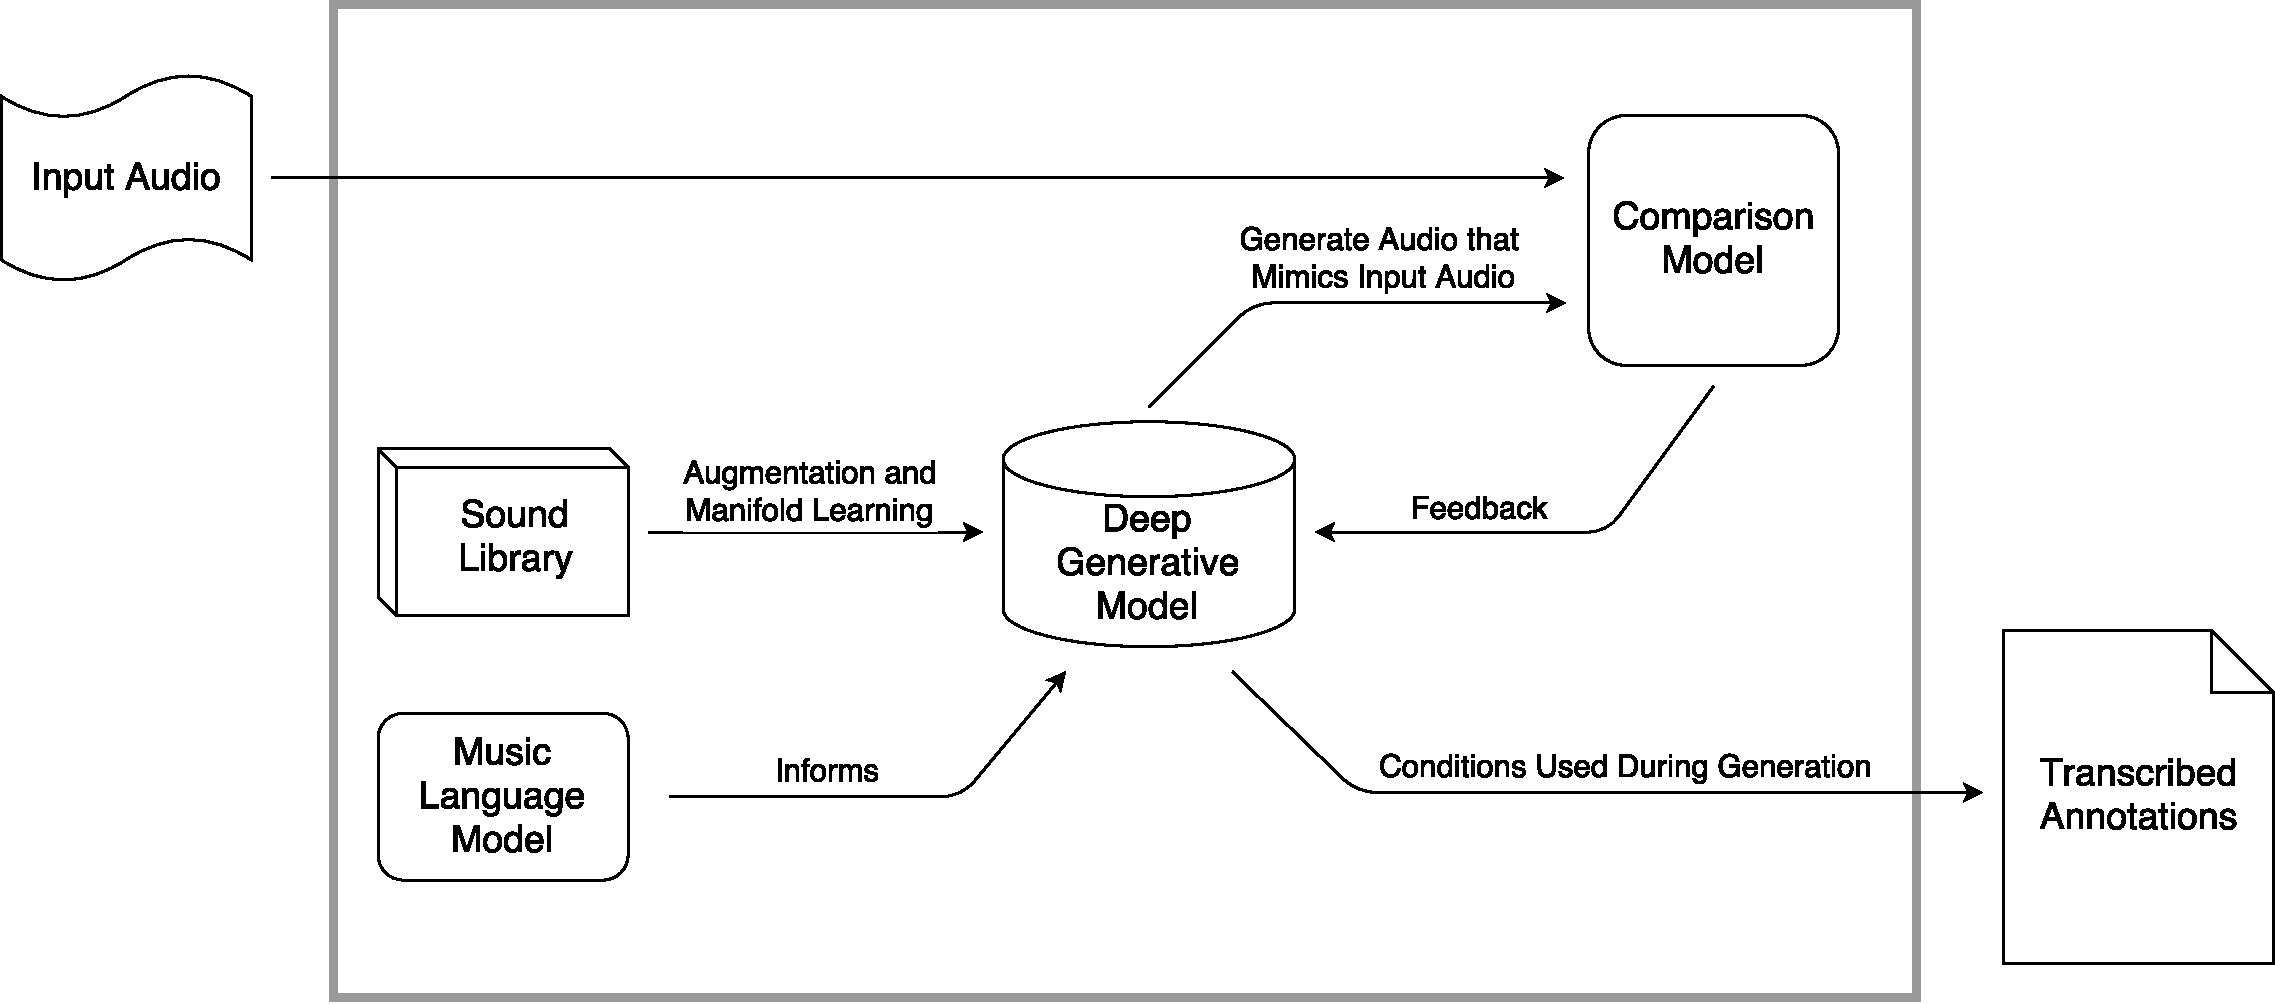
\includegraphics[width=\textwidth]{grand.pdf}
	\caption{A high-level schematic of the proposed automatic music transcription system. A deep generative model is trained using music database and music language models, to generate audio track that sounds similarly as the input audio. The conditions used to generate the matching audio can produce the predicted music transcription. }\label{fig:grand}
\end{figure}

Figure \ref{fig:grand} shows the high-level diagram for an end-to-end automatic music transcription system built around a deep generative model.
In short, the deep generative model in the center will learn to generate audio signals that mimics the input, and the combinations of instruments and pitches used for generating the audio will be the resulting transcription.
In order for the generative model to learn the semantic latent variables in music, the model needs to be able to disentangle the pitch and timbre information from the audio.
While the techniques such as batch normalization and using diagonal covariance matrices in variational autoencoders are intended to induce statistical independence between latent components,
making the components have a fully disentangled semantic information remains an active area of research.
The next section discusses the possible methods for disentanglement in the context of deep generative models.

%The proposed transcription system is not only powered by deep generative models and music language models, but also by a few other important techniques that will make the implementation possible to be realized.
%Data augmentation is a method for increasing the quantity of available data using transformations that does not alter or deterministically alter the label, and has been successfully applied to image classification tasks  \cite{krizhevsky2012imagenet}. MUDA \cite{mcfee2015muda} provides a software framework for augmenting musical audio, which supports pitch shift, time stretch, background noise, and dynamic range compression.
%It would be also possible augment to the data by filtering with the impulse responses according to various room acoustics, adding reverberations to the audio.
%Combined with the audio sources from various software instruments and sample libraries, these methods for audio augmentation can greatly increase the effective size of training data, and will help the deep model to more accurately learn the distribution of the real-world musical sounds.
%It is more efficient in terms of both time and space complexity to perform data augmentation on-the-fly instead of storing precomputed data, because the size of data increases combinatorially depending on the available augmentation schemes.


\section{Generative Models and Learning Disentangled Representations}

This section revisits the definition of generative model, whose primary focus is to model the data distribution:
\begin{equation}\label{eqn:data-distribution}
p(\mathbf{x}).
\end{equation}
The objective of AMT is to find the label (i.e. transcription) $\mathbf{y}$ corresponding to the data $\mathbf{x}$, in which case the generative model concerns the joint distribution of the data and the annotation:
\begin{equation}\label{eqn:joint-distribution}
p(\mathbf{x}, \mathbf{y}),
\end{equation}
as opposed to discriminative models which concerns the conditional distribution:
\begin{equation}\label{eqn:data-conditional-distribution}
p(\mathbf{y} | \mathbf{x}).
\end{equation}
Some deep generative models such as cGAN \cite{mirza2014conditional} can be formulated to perform a conditional generation depending on the label, effectively sampling from:
\begin{equation}\label{eqn:label-conditional-distribution}
p(\mathbf{x} | \mathbf{y}).
\end{equation}
Some may argue that this is not a true generative modeling, because the definition does not distinguish which among $\mathbf{x}$ and $\mathbf{y}$ is the label, so Equation \ref{eqn:label-conditional-distribution} should also describe a discriminative model as Equation \ref{eqn:data-conditional-distribution} does.

In this thesis, a relaxed definition of ``generative model'' will be used to classify those models as also generative, by distinguishing data and labels as:
\begin{itemize}
	\item \textbf{data}: a higher-dimensional entity that is typically observed as-is and consists of entangled representations from which it is harder to extract useful information.
	\item \textbf{label}: a lower-dimensional entity which often requires manual annotations to obtain and consists of disentangled representations from which it is easier to extract useful information.
\end{itemize}
By using this definition, a model that only performs conditional synthesis can still be called a generative model.

As emphasized in the introduction, disentanglement is the key to effectively obtaining the desired labels for AMT.
In the overview paper on representation learning, \citeA{bengio2013representation} concluded that the most robust feature learning should ``\emph{disentangle as many factors as possible, discarding as little information about the data as is practical}''.
The main hypothesis of this thesis is that generative models fit well to this objective, since they have to know all factors required for generation and have to minimize the information loss at the same time.
% The statical models for disentanglement are similar to the techniques for source separation covered in Section \ref{ch:mir}.\ref{sec:separation}, because source separation is essentially a disentanglement problem of different sources.
Deep learning models are considered to be doing particularly well in performing disentanglement, as they can learn high-level concepts from just pixel- or sample-level data examples.
\citeA{brahma2016disentanglement} studied the features learned in different layers in a deep model and observed that deeper layers gradually unfold and flatten the data distribution, building a disentangled representation.
However, it does not necessarily mean that the factors in deeper layers always contain completely isolated information of interest.

For this reason, inducing disentanglement in deep generative models has recently become an intriguing area of research.
InfoGAN \cite{chen2016infogan} is one of the most notable models that performs disentanglement in an unsupervised manner by maximizing the mutual information between a portion of latent factors and the observation.
Information dropout \cite{achille2018information} is a generalization of the standard Dropout technique that obtains more disentangled factors.
FactorVAE \cite{kim2018factor} is a VAE model that encourages the factors in variational posterior to be independent.
Other examples include DNA-GAN \cite{xiao2017dnagan} which is inspired by the mechanism of gene expression,
and semantically decomposed GAN (SD-GAN) \cite{donahue2017gan} which learns to distinguish variations in two domains by training with pairs of data examples belonging to the same category.

While there is no silver bullet yet, these studies suggest that principled considerations for achieving disentanglement should be made during the architectural design and experiments for this thesis.


\section{Methods}

This section describes the methodology and the experimental design for achieving the goals of this thesis.
There are two main subproblems defined in Section \ref{ch:introduction}.\ref{sec:subproblems}, concerning AMT using a deep generative model and using the generative component for data augmentation.
The experiments for each subproblem are designed to follow the corresponding lower-level questions, which is aimed at incrementally getting closer to the final goals.

\subsection{End-to-End Generative Model between Audio and Piano Rolls}

This task is the primary objective of this thesis, by building a bidirectional connection between the domain of audio signals and the domain of piano roll representations.
The three subtasks are designed to gradually expand the two domains, from a fixed-length monophonic notes to multi-instrument polyphonic music.

\paragraph{Disentangling Pitch and Timbre}\mbox{}

For the first subtask, fixed-length monophonic signals are assumed.
As \citeA{engel2017nsynth} studied the entanglement of pitch and timbre using the WaveNet architecture, the goal of this subtask is to build a deep generative model that can separately control pitch and timbre.
A preliminary architecture implementing this idea is shown in Figure \ref{fig:pegan}.
Domain-adversarial training \cite{ganin2015domain} and semantically decomposed GAN \cite{donahue2017gan} could be helpful in stable training of the proposed setup.
A shortcoming of this architecture is that each pitch values are considered as separate categories, and it could be overcome by an improved methods for conditional synthesis, such as the projection discriminator \cite{miyato2018cgan}.

\begin{figure}
	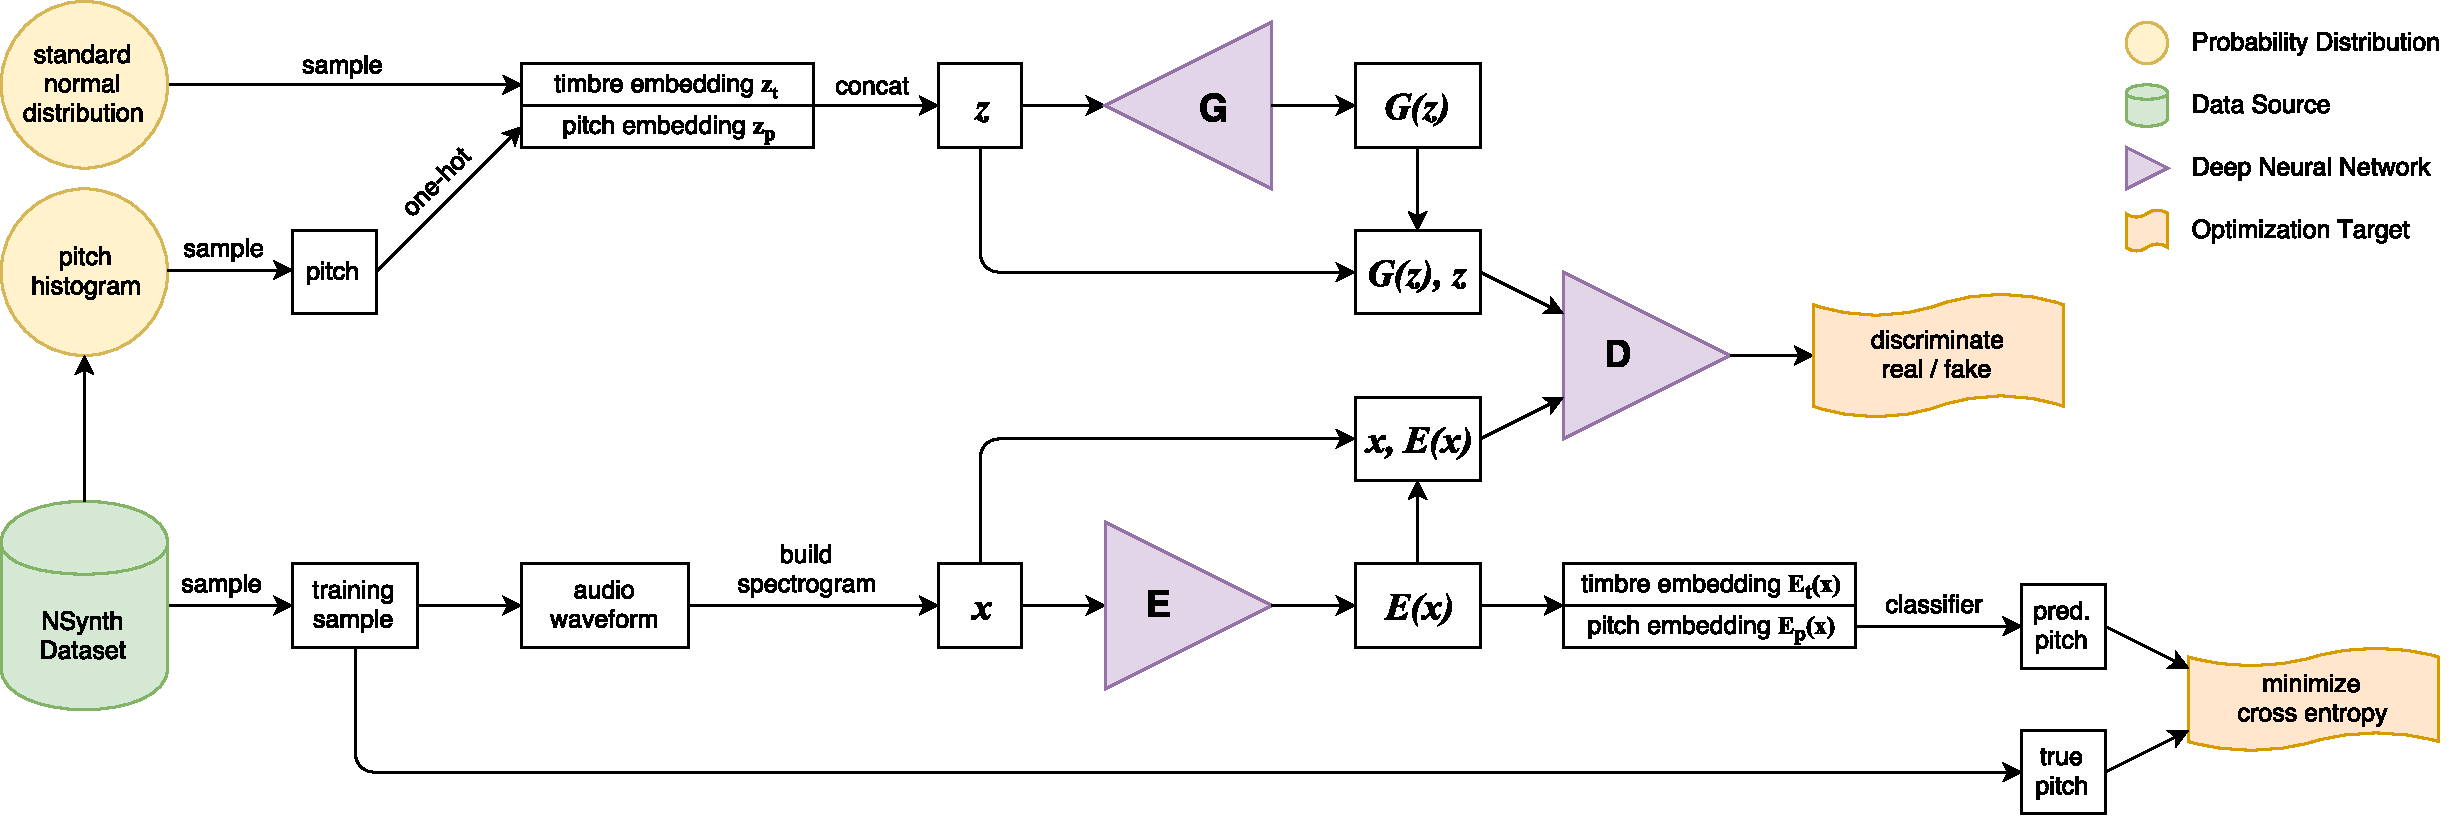
\includegraphics[width=\textwidth]{PEGAN.pdf}
	\caption{An architecture combining a conditional GAN \protect\cite{mirza2014conditional} and a bidirection GAN \protect\cite{donahue2016bigan}, which uses a concatenation of pitch and timbre embeddings to be able to control pitch and timbre separately in the generator.}
	\label{fig:pegan}
\end{figure}

\paragraph{Extending to Polyphony and Variable-Length Audio}\mbox{}

The next goal is to extend the generative model to deal with polyphony and variable-length audio.
In order to generalize to an arbitrary length in time, the latent representation needs to include the time dimension in addition to the pitch and timbre factors.
This is in a similar manner where \citeA{engel2017nsynth} used a generative model trained on 4-second clips to synthesize audio of a longer length.
The fully convolutional architecture \cite{shelhamer2017fcn} may be appropriate for dealing with variable-length inputs and outputs.

In order for the model to learn to separate different timbres and pitches, the transcription model may contain an addition operation which mixes multiple sources corresponding to each instrument and each note.
Such setup may not have a straightforward training scheme, in which case incorporating a clustering techniques such as expectation-maximization can be helpful.
It may be also necessary to limit the number of polyphony or instruments to have a computationally feasible solution.

\paragraph{Obtaining Piano Rolls from the Embeddings}\mbox{}

This task is on the ultimate problem of obtaining the per-instrument piano roll representations.
In order to achieve this, a model connecting the event-level representation to the latent embedding space is required.

\subsection{Generative Model as Augmentation}

This subproblem concerns the secondary objective of this thesis, of using the generative component of the AMT model for data augmentation.
These tasks are auxiliary to the main objective and are also less technically challenging, while they are designed to work in conjunction with the AMT model.

\paragraph{Software Instrument and Audio Post-Processing}\mbox{}

This task is to reconfirm the effectiveness of data augmentation, by feeding additional training dataset consisting of sounds generated using software instruments and audio post-processing techniques.
While the audio degradation toolbox \cite{mauch2013adt} and MUDA \cite{mcfee2015muda} could provide some facilities for data augmentation, software instruments are usually packaged using specialized APIs, such as VST3 or Audio Units \cite{pirkle2014synthesizer}.

In some sense, by building a generative model based on a specific dataset, the model essentially serves as a software instrument.


\paragraph{Incorporating a Music Language Model}\mbox{}

This subtask concerns the application of a music language model that serves as a sensible prior to the output of the generative AMT model.
Designing a music language model itself is an intriguing problem, but for the purpose of this thesis, existing music sequence generation models such as MidiNet \cite{yang2017midinet} or MuseGan \cite{dong2017musegan} can be incorporated.

\paragraph{Positive Feedback Cycle between Transcription and Augmentation}\mbox{}

This last task would be an integration of all of the above methods, to build an architecture where the improved generative model serves as a better augmentation tool, which helps the AMT model achieve improved transcription performance.


\subsection{Expected Challenges}

Regretfully, the above descriptions of the experimental designs do not fully specify the model architecture and representation, because the biggest challenges lie on finding the exact architecture and representation that works.
One such challenge is the size of the representation; generative adversarial networks are the only deep generative models that have meaningfully generated images larger than 128$\times$128 pixels, however the training dynamics of GANs become increasingly unstable as the size of the representation gets larger.
In order to train a GAN that deals with a sufficient size of audio representation, it may be necessary to employ more intricate architecture such as progressive growing \cite{karras2017pggan}.
Another obstacle is the flood of GAN models, making it even more difficult to determine the correct architecture to work with.
Deeper theoretical understanding and empirical knowledge on GAN training would be required.

\section{Evaluation}

The performance of multiple fundamental frequency estimation in the form of piano rolls are evaluated in a number of different ways.
The simplest metric is the frame-level accuracy, which measures the portion of the correct predictions 
\begin{equation}
\mathrm{Accuracy} = \frac{\sum_{t=1}^T TP(t)}{\sum_{t=1}^T \left ( TP(t) + FP(T) + FN(t) \right ) },
\end{equation}
where TP, FP, and FN refers to true positives, false positives, and false negatives, respectively.

Additional evaluation metrics have been proposed in \cite{poliner2007piano} to reflect three different types of transcription errors, a missed error where the system fails to predict a pitch at all, a substitution error where a different F0 is predicted, and a false alarm where the system predicts a pitch that is not actually present:
\begin{eqnarray}
E_{tot} & = & \frac{\sum_{t=1}^T \max ( N_{ref}(t), N_{sys}(t) ) - N_{corr}(t)}{\sum_{t=1}^T N_{ref}(t)}, \\
E_{sub} & = & \frac{\sum_{t=1}^T \min ( N_{ref}(t), N_{sys}(t) ) - N_{corr}(t)}{\sum_{t=1}^T N_{ref}(t)}, \\
E_{miss} & = & \frac{\sum_{t=1}^T \max ( 0, N_{ref}(T) - N_{sys}(t) )}{\sum_{t=1}^T N_{ref}(t)}, \\
E_{fa} & = &  \frac{\sum_{t=1}^T \max ( 0, N_{sys}(T) - N_{ref}(t) )}{\sum_{t=1}^T N_{ref}(t)},
\end{eqnarray}
where $N_{ref}(t)$ the number of ground-truth f0s at frame $t$, $N_{sys}$ is the number of reported f0s, and $N_{corr}(t)$ is the number of correctly predicted f0s.
These errors are useful, because they enable a comparison of multi-pitch estimation systems with respect to the different types of errors \cite{bay2009evaluation}.
The open-source implementation in the \texttt{mir\_eval} package \cite{raffel2014mir_eval} will be used for convenience and reproducibility.

\section{Datasets}

In order to comply with the assumptions on the scope of music discussed in Section \ref{ch:introduction}.\ref{sec:limitations}, datasets that contain non-vocal harmonic instrumental sounds without excessive variations in timbre are desirable.
For early experiments, the NSynth Dataset published recently by Google's Magenta project \cite{engel2017nsynth} is appropriate, as the dataset contains additional kinds of instruments and comes with more accurate annotations.
As discussed above, open-source and commercial software instruments and effects can also be used.

In order to compare the performance of the proposed AMT model with existing transcription methods, the standard benchmark datasets containing polyphonic classical instruments such as MAPS \cite{emiya2010multipitch}, Bach10 \cite{duan2010bach10}, and MusicNet \cite{thickstun2017musicnet} are good choices.
